
\subsection{Diffusion of Technology}\label{subsec:techDiffusion}



\ifInBook{}{
%\begin{center}	[Insert Figure \ref{fig:graph_diffusion}  here]\end{center}

\begin{figure}[!ht] \centering  % [h!]
	\caption{ ~Literature map of EE models of technological diffusion}
	\label{fig:graph_diffusion}
	\centerline{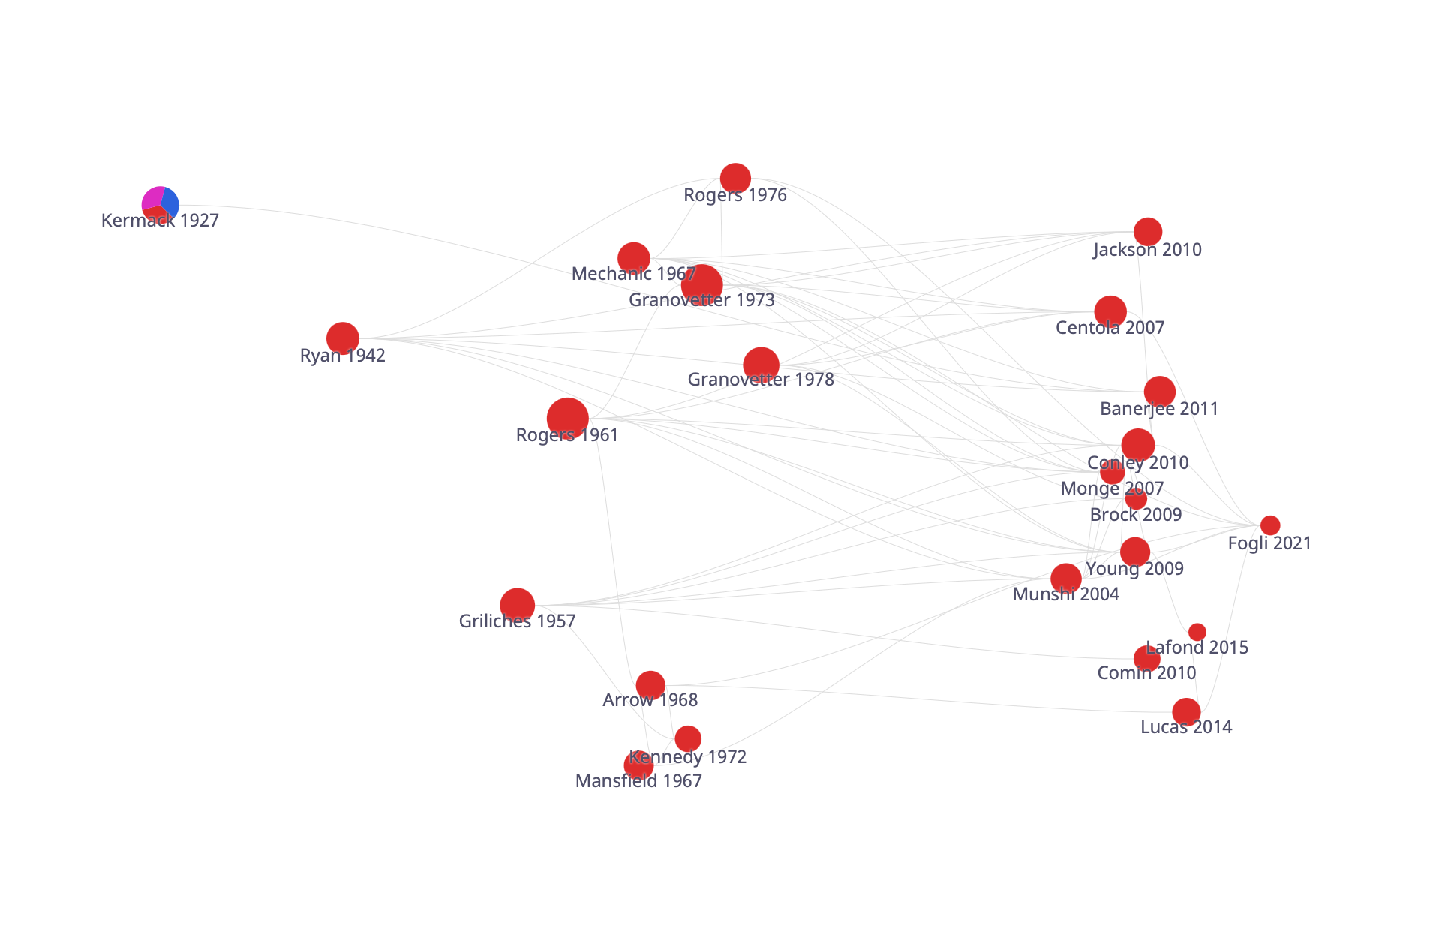
\includegraphics[width=\textwidth]{./figures/graph_diffusion}}
	\begin{flushleft}
		{\footnotesize Note: This graph includes selected papers under the topic of epidemiological modeling of technological/innovation diffusion in economics and closely related literature from other fields. See \href{https://app.litmaps.co/shared/1D9003CB-75FE-4633-B60A-79B70E03B691}{here} for an interactive version.}
	\end{flushleft}
\end{figure}

}

%Economists have understood since \cite{solow1956contribution} that technological progress is the wellspring of economic growth.  Although in studies of the process by which fundamentally new technical knowledge is generated, we are not aware work that could be classified as epidemiological, the vast bulk of technological progress for most of the individual agents who are progressing does not reflect their independent invention of ideas novel to humanity -- it reflects their adoption of knowledge invented by others.  In recognition of this fact, an extensive literature has studied a topic usually identified as `the diffusion of technology.'  Traditionally, this line of work has been seen as separate from the domain of economic expectations.  But the reason for adopting a new technology is surely that there is an expected gain from doing so, a point that is explicitly made at various places in the more theoretically-minded branches of the literature.

% draws an explicit analogy between the diffusion of ideas and the spread of disease.  %(His paper is one of the earlier contributions from the economics literature; see Section~\ref{subsec:nonecon} for work outside of economics on the diffusion of scientific knowledge.)
\IfPrivate{\href{https://github.com/iworld1991/EpiExp/blob/master/Literature/arrow_classificatory_1969.pdf}{\cite{arrow_classificatory_1969}}}{\cite{arrow_classificatory_1969}} argues that the process of knowledge diffusion may account for international differences in both levels and dynamics of income per capita. He conjectures that knowledge diffusion is influenced by factors that he explicitly compares to  those that influence the spread of disease including (1) the perceived reliability of the sender (which affects infectiousness); (2) socioeconomic traits (which affect exposure and susceptibility); (3) the understandability of information by the receiver (degree of immunity); and so on.

Arrow's interpretation puts technological diffusion squarely in the realm of EE modeling, under the mild further assumption that what spreads is the `expectation' that adoption of the technology will yield higher productivity (See \cite{banerjee2013diffusion}, discussed below, for survey evidence confirming that people adopt a technology when they expect it to be beneficial).

In closely related work, \IfPrivate{\href{https://en.wikipedia.org/wiki/Diffusion_of_innovations}{\cite{rogers1962diffusion}}}{\cite{rogers1962diffusion}} popularized a theory of the ``diffusion of innovations'' based on a meta-analysis of studies of the spread of ideas in academic disciplines.\footnote{Though Rogers was a sociologist, we include his work in the discussion here because it has had such a strong impact on the subsequent economics literature.}  The factors that this literature identifies as determinants of the dynamics of diffusion are directly interpretable as corresponding to the ``infectiousness'' of the idea, the degree to which populations are ``exposed'' to the idea, and many of the other elements of epidemiological models.

\IfPrivate{\href{https://github.com/iworld1991/EpiExp/blob/master/Literature/young2009innovation.pdf}{\cite{young2009innovation}}}{\cite{young2009innovation}} presents a broad survey of how alternative epidemiological models generate different shapes of  ``adoption curves'' with consequent effects on the path of economic growth. He shows how the shape of diffusion curves differs in models of `inertia' (a SI common-source model), `social influence' (a threshold model), `contagion' (a transmissible SI model), and `social learning,' where learning is based on observed actions of others.\footnote{We do not survey a large parallel literature on technology/innovation diffusion in economics that features the role of social learning, as this work is not explicitly built upon epidemiological frameworks. Examples include  \cite{munshi2004social},  \cite{comin2010exploration} and so on.}  % the first one is field evidence on tech diffusion in Indian showing that information flow is weaker when  underlying hterogeneity is higher.  The scond  builds the process of tech diffusion  into a neocalssical growth model.


The aforementioned  \IfPrivate{\href{https://pubmed.ncbi.nlm.nih.gov/23888042/}{\cite{banerjee2013diffusion}}}{\cite{banerjee2013diffusion}} estimates an epidemiological model based on the real-world network and pattern of  diffusion of microfinance in Indian villages, providing direct evidence for word-of-mouth diffusion of beliefs through a social network. %The model differentiates between agents who simply adopt the technology because they have heard about it from others (an `information passing mechanism') and those who have adopted due to others' participation (an `endorsement mechanism'). This is an example of how standard epidemiological models can be extended to incorporate alternative infection rules to accommodate more sophisticated applications.

\cite{lucas2014knowledge} construct an economy containing agents with a distribution of levels of productivity, and consider the dynamics of aggregate productivity under several alternative assumptions about how agents with lower productivity `learn' from agents with higher productivity.  %(`Learning' just means that, in an encounter between two agents, the agent with lower productivity adopts the other agent's technology).  %Encounters between agents are of the standard epidemiological `random mixing' kind.
% The baseline version of the model is one in which every agent is eligible to adopt any technology they encounter, which corresponds roughly to an epidemiological assumption that the `disease' is equally transmissible to all agents.  They also consider an alternative in which it is easier to move to a technology that is `near' your own than to leap across a large technological gap.  This latter assumption can perhaps be thought of as being similar to the `threshold' mechanisms discussed above, in which an idea is more likely to be transmitted if an agent is exposed to it many times -- assuming that agents are more likely to encounter other agents whose productivity levels are similar to their own.
Agents solve an optimization problem to determine the intensity of their search effort, which affects the likelihood of encountering an agent with a learnable ``better technology.''  %; this framework is constructed so that the agents have enough knowledge of the productivity distribution (and the efficacy of search) to make such choices rationally.
\ifInBook{}{
This is likely to be a common direction in which economists may take epidemiological models: Incorporation of purposive behaviors by agents. While some work in epidemiology allows agents to take actions to reduce the probability of infection, models in that literature have rarely been formulated with an eye to creating a structure where an explicit analytical optimization problem can be stated and solved.}

% CDC: this is where Lucas and Moll's paper should be surveyed.
% Abstract:  We analyze a model economy with many agents, each with a differ- ent productivity level. Agents divide their time between two activi- ties: producing goods with the production-related knowledge they already have and interacting with others in search of new, productivity- increasing ideas. These choices jointly determine the economy’s cur- rent production level and its rate of learning and real growth. We construct the balanced growth path for this economy. We also study the allocation chosen by an idealized planner who takes into account and internalizes the external benefits of search. Finally, we provide three examples of alternative learning technologies and show that the prop- erties of equilibrium allocations are quite sensitive to two of these var- iations.

% Conclusion We have proposed and studied a new model of economic growth in which individuals differ only in their current productivity, and the state of the economy is fully described by the probability distribution of pro- ductivities. The necessary conditions for equilibrium in the model take the form of a Bellman equation describing individual decisions on the way to allocate time between producing and searching for new ideas and a law of motion for the economywide productivity distribution. With the right kind of initial conditions, these forces can interact to generate sustained growth. We show that among these possibilities is a balanced growth path, characterized by a constant growth rate and a stable Lorenz curve describing relative incomes. We provide an algorithm for calcu- lating solutions along this path. This solution is the outcome of a decentralized system in which each agent acts in his own interest. But the new knowledge obtained by any one agent benefits others by enriching their intellectual environment and raising the return to their own search activities. We then formulate the problem of a hypothetical planner who can allocate people’s time so as to internalize this external effect. We show how the decentralized algorithm can be adapted to compute the planning solution as well and compare it to the decentralized solution. We then consider tax struc- tures that implement an optimal solution. Finally, we provide three ex- amples of alternative learning technologies and show that the properties of equilibrium allocations are quite sensitive to these variations. All of this is carried out in a starkly simple context in order to reveal the economic forces involved and the nature of their interactions and to build up our experience with a novel and potentially useful mathemat- ical structure. But we also believe that the external effects we study here are centrally important to the understanding of economic growth and would like to view our analysis as a step toward a realistically quantitative picture of the dynamics of production and distribution.17

% Other quotes: The learning technology involves random meetings: Each person meets others at a rate that depends on the fraction of time he spends in search. For us, a meeting means simply an observation of someone else’s productivity. If that productivity is higher than his own, he adopts it in place of the productivity he came in with. Everyone’s productivity level is simply the maximum of the productivities of all the people he has ever met. To ensure that the growth generated by this process can be sustained, we add an assumption to the effect that the stock of good ideas waiting to be discovered is inexhaustible.

%  In Section VI, we make use of this fact and explore three alternative learning technologies. The first variation we consider is one in which agents learn from an outside idea source as well as from others in the economy. One might describe this as a combination of “innovation” and “imitation,” but we will show that the asymptotic behavior of the productivity distribution in the modified model is observationally equivalent to that in our simpler, benchmark model. Next we consider a substantively more interesting model in which there are limits to learning in the sense that recipients of ideas can learn from donors only if their knowledge levels are not too differ- ent. Finally, we explore an alternative assumption regarding the symme-try of meetings, that is, who can learn what from whom depending on who initiated a meeting. It turns out that the properties of equilibrium allocations are quite sensitive to these last two variations, which is to say that different assumptions on technology diffusion that cannot be tested by direct observation may have very different implications for the behavior of observables.1 For example, with limits to learning, un- productive individuals no longer exert more search effort than produc- tive ones, and search effort is now a nonmonotonic function of pro- ductivity.

Not only are mechanisms of the spread of technology and disease comparable, they may interact.  \IfPrivate{\href{https://github.com/iworld1991/EpiExp/blob/master/Literature/fogli2012germs.pdf}{\cite{fogli2021germs}}}{\cite{fogli2021germs}} develop a model in which the structure of the networks connecting people (`nodes') allows the authors to explore the roles of the three dimensions central to the network theory literature that has developed since \cite{erdos1960evolution}: `degree,' `clustering,' and `sprinkling' (see section~\ref{subsec:epiNet}).  Both productivity and disease spread through these connections, so the dynamics of productivity and disease are connected.  The model highlights a trade-off between the speed of technological diffusion and disease spreading, which affect economic growth outcomes in opposite directions.

%For example, although the authors do not put it in quite this way, one implication of the model is that a bright side of the spread of disease is that the deceased are replaced by higher-productivity nodes.%  (The authors perhaps do not intend for the reader to take all the paper's policy implications at face value.)

% CDC: I felt we did not emphsize the central message of the paper: the trade-off between high degree of diffusion of the technology and disease.
